\section{A new approach}
As pointed out by the RxJava wiki \cite{RxJava-Wiki-Backpressure}, backpressure does not make the problem of an overproducing source go away. It only moves the problem up the chain of operators to a point where it can be handled better. This means that a \code{request(n)} call from the \code{zip} operator in section~\ref{sec:fastproc-slowcons} goes up the chain to the point where it can fulfill that request. This is either an operator or the source that is wrapped in an \code{Observable.create} or one of its higher abstractions.

In our opinion RxJava did not go far enough with this approach. We think it is better to decouple the flow control from the operators and move it to the source of the stream. This way we can keep the API clean, we do not have to take this flow control into account while implementing new operators, we do not have to reimplement operators for this and (most importantly) we can keep the operator sequences reactive. Obviously RxJava cannot be used for this, as it already has a backpressure implementation. Therefore we will use the RxMobile \cite{RxMobile} reference implementation that was recently written in Scala by Erik Meijer as a basic API for reactive programming and build on top of that to support backpressure without rewriting any existing code.

In order to do so, we need to observe where the \obs comes from. In essence, it is nothing more than a source wrapped in \code{Observable.create}, from which it inherits all the operators and for the RxJava implementation also inherits the possibility to apply backpressure. This wrapped source can then be used as the origin of an \obs sequence or it might be returned by an operator like \code{flatMap}.

Instead of wrapping a cold source in the \code{Observable.create}, we want to wrap it in an interactive interface (such that communication with the source is not coupled with its own specific interface) and pull the data out of the source via this interface. We will then add these values to a bounded buffer, from which they are pulled again by a downstream \obs on another thread. Once an element is pulled from the buffer, it will block the downstream \obs's callstack from pulling another element until the current element is fully processed or taken over by another thread. In the mean time the buffer request new elements from the source and by doing so keeps the downstream \obs as busy as it possibly can.

\begin{figure}[H]
	\begin{center}
		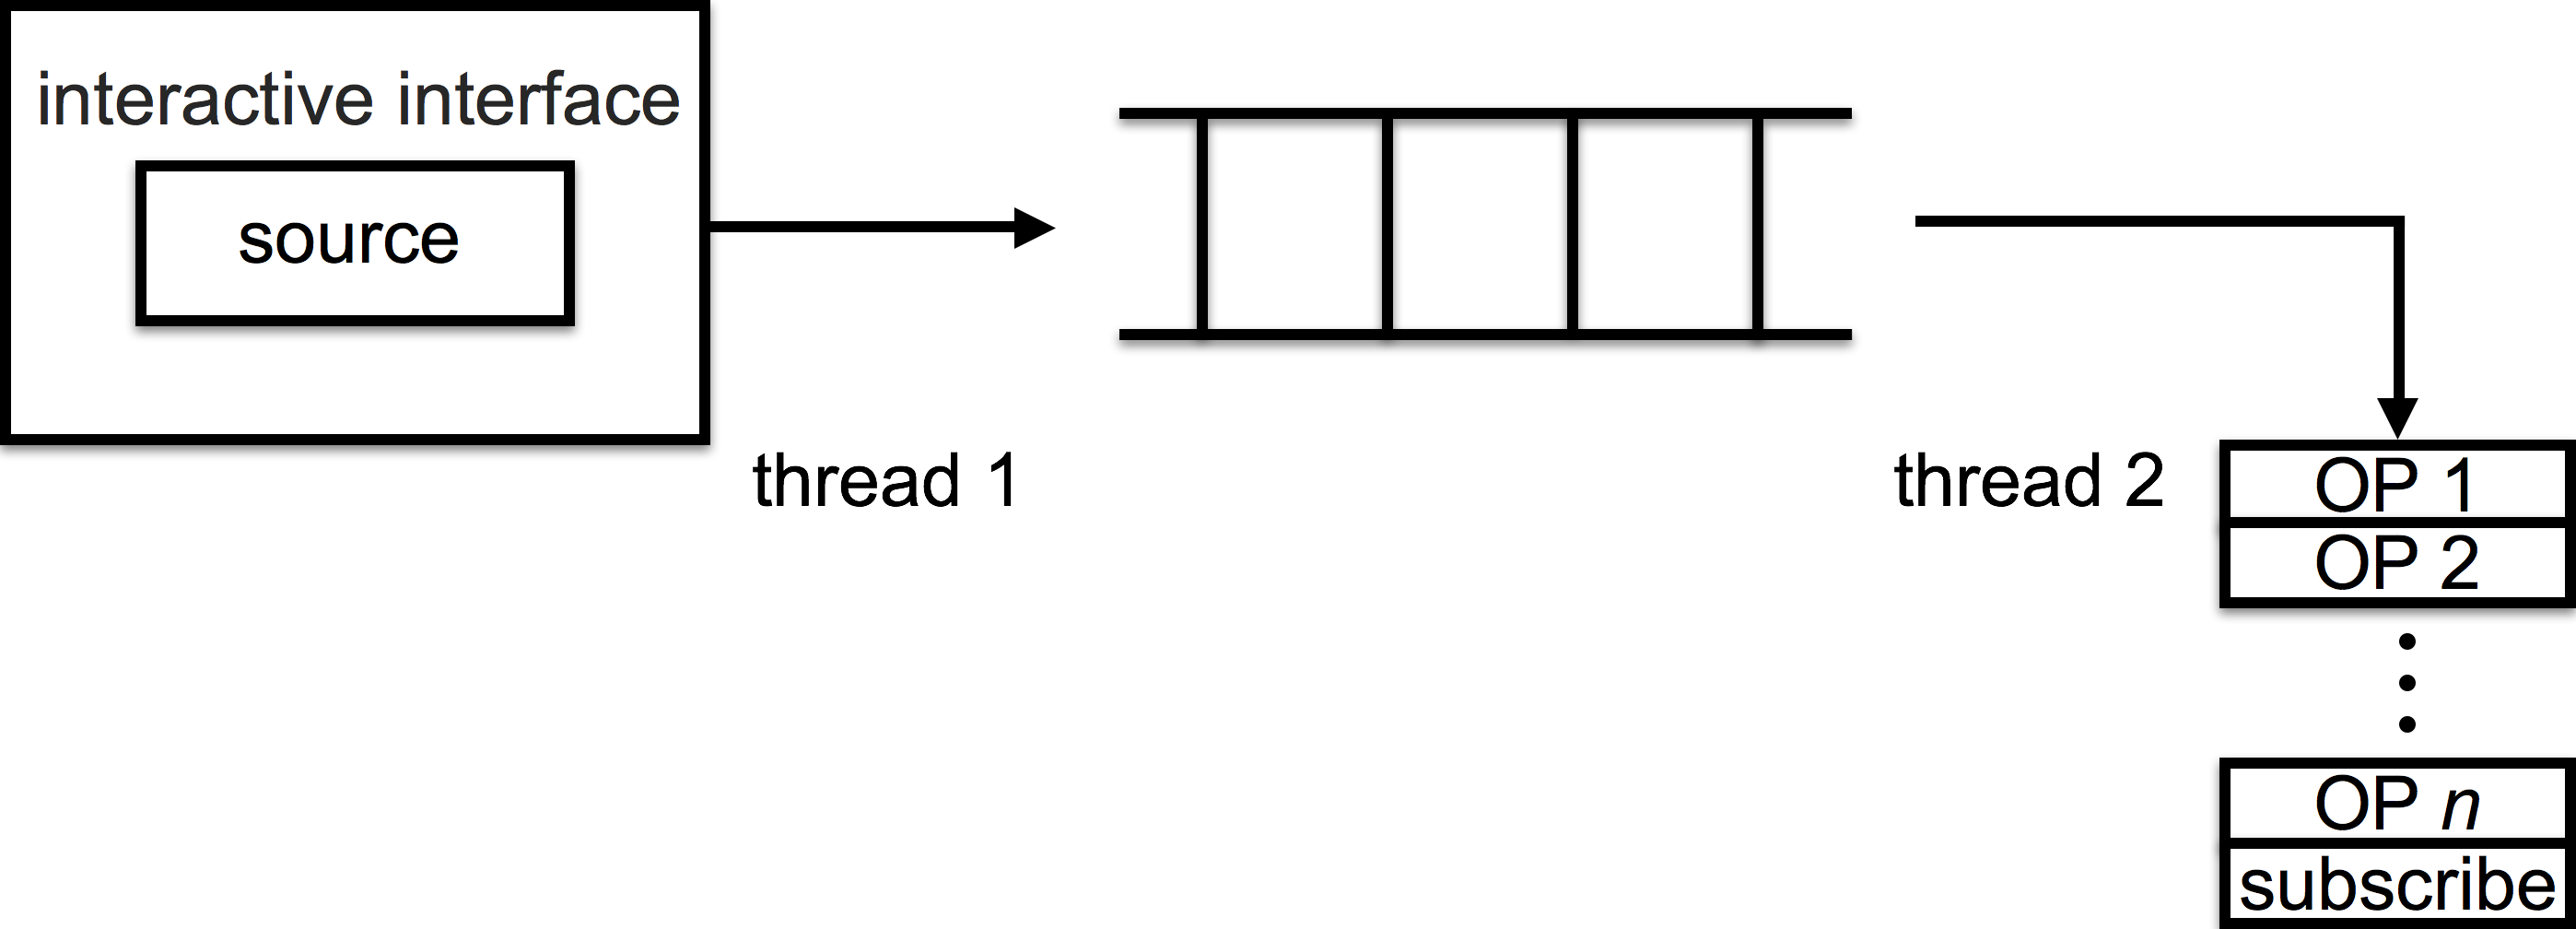
\includegraphics[width=0.65\textwidth]{figures/Approach.png}
	\end{center}
	\label{fig:new-approach}
	\caption{Schematic representation of our approach}
\end{figure}

With this approach we have reduced the problem of overproduction to a problem of controlling the size of a buffer to be as small as possible, without the buffer being exhausted by a fast consuming downstream. A buffer size that is too small can lead to a needless delay in consuming the data, whereas a too large buffer size is not desirable as well, given that we want to spend as little resources as possible. The complicating factor here is that it is unknown at all times how long it will take for the source to produce a next element.

In order to overcome this unknown factor, control the size of the buffer and only request new elements from the source when needed, we will use a well-known technique from mechanical and electrical engineering called \textit{feedback control}. Since this is a technique that is unfortunately not as well-known in computer science and software engineering as it is in other parts of science and engineering, we will introduce this technique in the upcoming chapters, develop an API to work with this technique in general and present the rest of our solution to the overproduction problem after that.
